\label{ap:ap15}
\chapter{Tópicos em IA}
\section*{\textbf{A - ENUNCIADO}}

\subsection*{\textbf{1 Algoritmo Genético}}


\textcolor{black}{Problema do Caixeiro Viajante}


\textcolor{black}{A Solução poderá ser apresentada em: Python (preferencialmente), ou em R, ou em Matlab, ou em C ou em
Java.}


\textcolor{black}{Considere o seguinte problema de otimização (a escolha do número de 100 cidades foi feita simplesmente
para tornar o problema intratável. A solução ótima para este problema não é conhecida).}


\textcolor{black}{Suponha que um caixeiro deva partir de sua cidade, visitar clientes em outras 99 cidades diferentes, e
então retornar à sua cidade. Dadas as coordenadas das 100 cidades, descubra o percurso de menor distância que passe uma
única vez por todas as cidades e retorne à cidade de origem.}


\textcolor{black}{Para tornar a coisa mais interessante, as coordenadas das cidades deverão ser sorteadas (aleatórias),
considere que cada cidade possui um par de coordenadas (x e y) em um espaço limitado de 100 por 100 pixels.}


\textcolor{black}{O relatório deverá conter no mínimo a primeira melhor solução (obtida aleatoriamente na geração da
população inicial) e a melhor solução obtida após um número mínimo de 1000 gerações. Gere as imagens em 2d dos pontos
(cidades) e do caminho.}


\textcolor{black}{Sugestão: }
\begin{enumerate}[series=listWWNumxxiii,label=(\arabic*),ref=\arabic*]
\item \textcolor{black}{considere o cromossomo formado pelas cidades, onde a cidade de início (escolhida aleatoriamente)
deverá estar na posição 0 e 100 e a ordem das cidades visitadas nas posições de 1 a 99 deverão ser definidas pelo
algoritmo genético.}
\item \textcolor{black}{A função de avaliação deverá minimizar a distância euclidiana entre as cidades (os pontos).}
\item \textcolor{black}{Utilize no mínimo uma população com 100 indivíduos;}
\item \textcolor{black}{Utilize no mínimo 1\% de novos indivíduos obtidos pelo operador de mutação;}
\item \textcolor{black}{Utilize no mínimo de 90\% de novos indivíduos obtidos pelo método de cruzamento (crossover-ox);}
\item \textcolor{black}{Preserve sempre a melhor solução de uma geração para outra.}
\end{enumerate}

\textbf{\textcolor{black}{Importante}}\textcolor{black}{: A solução deverá implementar os operadores de “cruzamento” e
“mutação”.}


\subsection*{\textbf{2 Compare a representação de dois modelos vetoriais}}


\textcolor{black}{Pegue um texto relativamente pequeno, o objetivo será visualizar a representação vetorial, que poderá
ser um vetor por palavra ou por sentença. Seja qual for a situação, considere a quantidade de palavras ou sentenças
onde tenha no mínimo duas similares e no mínimo 6 textos, que deverão produzir no mínimo 6 vetores. Também limite o
número máximo, para que a visualização fique clara e objetiva.}


\textcolor{black}{O trabalho consiste em pegar os fragmentos de texto e codificá-las na forma vetorial. Após obter os
vetores, imprima-os em figuras (plot) que demonstrem a projeção desses vetores usando a PCA.}


\textcolor{black}{O PDF deverá conter o código-fonte e as imagens obtidas.}


%%%%%%%%%%%%%%%%%%%%%%%%%%%%%%%%%%%%%%%%%%%%%%%%%%%%%%%%%%%%%%%%%%%%%%%%%%%%%%%%%%%%%%%%%%%%%
\section*{\textbf{B - RESOLUÇÃO}}


\subsection*{\textbf{1 Algoritmo Genético}}

Importações

\begin{lstlisting}[language=Python, style=input]
import numpy as np
import matplotlib.pyplot as plt
import random
from itertools import permutations
\end{lstlisting}

Configurações

\begin{lstlisting}[language=Python, style=input]
NUM_POPULACAO = 100
GERACOES = 1000
TAXA_MUTACAO = 0.01
TAXA_CRUZAMENTO = 0.9
\end{lstlisting}

Gerar cidades aleatórias

\begin{lstlisting}[language=Python, style=input]
cidades = np.random.rand(NUM_POPULACAO, 2) * 100
def populacaoInicial(tamanho): 
    resultado = [] 
    for \_ in range(tamanho): 
        individuo = list(np.random.permutation(NUM_POPULACAO)) 
        resultado.append(individuo) 
    return resultado
\end{lstlisting}

Desenha solução encontrada

\begin{lstlisting}[language=Python, style=input]
#def printaSolucao(caminho, titulo):
# cidadesOrdenadas = np.append(caminho, caminho[0])
# plt.figure(figsize=(10, 6))
# plt.scatter(cidades[:, 0], cidades[:, 1], c='red')
# plt.plot(cidades[cidadesOrdenadas, 0], cidades[cidadesOrdenadas, 1], 'b-')
# plt.title(titulo)
# plt.show()
def printaSolucao(caminho, titulo): 
    cidadesOrdenadas = caminho + [caminho[0]] 
    plt.figure(figsize=(12, 8)) 
    plt.scatter([c[0] for c in cidades], [c[1] for c in cidades], c='red', s=50, label="Cidades") 
    plt.plot([cidades[i % NUM_POPULACAO][0] for i in cidadesOrdenadas], [cidades[i % NUM_POPULACAO][1] for i in cidadesOrdenadas], 'b-', alpha=0.6, linewidth=1.5) 
    for i, (x, y) in enumerate(cidades): 
        plt.text(x, y, str(i), fontsize=9, ha='right', color='black') 
    plt.xlim(-10, 110) 
    plt.ylim(-10, 110) 
    plt.grid(True, linestyle='--', alpha=0.5) 
    plt.title(titulo) 
    plt.legend() 
    plt.show()
\end{lstlisting}

Calculos distâncias
\begin{lstlisting}[language=Python, style=input]
    def distanciaEuclidiana(a, b): 
        return np.linalg.norm(a - b)
#def distanciaEuclidiana(a, b):
# return np.sqrt((a[0] - b[0])**2 + (a[1] - b[1])**2)
def distanciaTotal(caminho): 
    distancia = 0 
    for i in range(len(caminho) - 1): 
        distancia += distanciaEuclidiana(cidades[caminho[i]], cidades[caminho[i+1]]) 
    distancia += distanciaEuclidiana(cidades[caminho[-1]], cidades[caminho[0]]) 
    return distancia
\end{lstlisting}

implementa cruzamento
\begin{lstlisting}[language=Python, style=input]
def cruzamento(pai, mae): 
    inicio, fim = sorted(random.sample(range(NUM_POPULACAO), 2)) 
    filho = [-1] * NUM_POPULACAO 
    filho[inicio:fim] = pai[inicio:fim] 
    ptr = fim 
    for gene in mae:
       if gene not in filho: 
           while filho[ptr % NUM_POPULACAO] != -1: 
               ptr += 1 
           filho[ptr % NUM_POPULACAO] = gene 
    return np.array(filho)
\end{lstlisting}

Implementa mutação

\begin{lstlisting}[language=Python, style=input]
def mutacao(individuo): 
    if random.random() < TAXA_MUTACAO: 
        i, j = random.sample(range(NUM_POPULACAO), 2) 
        individuo[i], individuo[j] = individuo[j], individuo[i] 
    return individuo
\end{lstlisting}

Implementa seleção

\begin{lstlisting}[language=Python, style=input]
def selecao(populacao, fitness): 
    total = sum(fitness) 
    probabilidades = [a / total for a in fitness] 
    idx1, idx2 = random.choices(range(len(populacao)), weights=probabilidades, k=2) 
    return populacao[idx1], populacao[idx2]
\end{lstlisting}

Inicialização

\begin{lstlisting}[language=Python, style=input]
populacao = populacaoInicial(NUM_POPULACAO)
melhorSolucao = min(populacao, key=distanciaTotal)
melhorDistancia = distanciaTotal(melhorSolucao)
printaSolucao(melhorSolucao, "Solução Inicial Aleatória")
\end{lstlisting}

\begin{figure}[H]
\centering
\caption{Solução Inicial Aleatória}
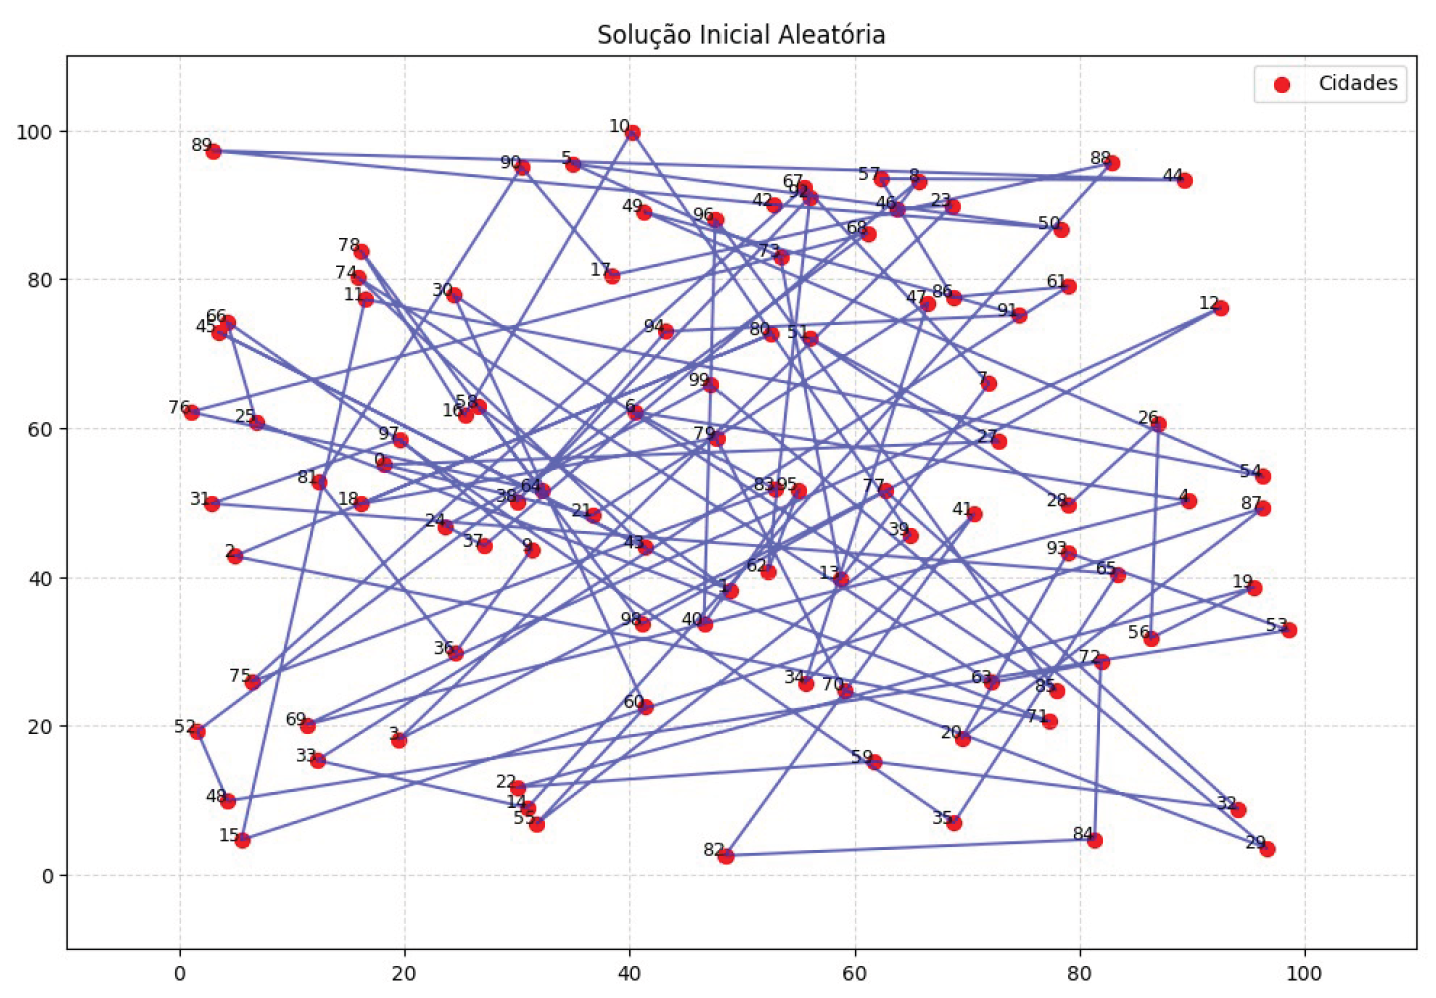
\includegraphics[width=1\linewidth]{apendices/fig/IAA015_1.png}
\caption*{Fonte: O autor (2025).}
\end{figure}

Algoritmo Genético

\begin{lstlisting}[language=Python, style=input]
for geracao in range(GERACOES): 
    fitness = np.array([1 / distanciaTotal(ind) for ind in populacao])
    novaPopulacao = [melhorSolucao]
    while len(novaPopulacao) < NUM_POPULACAO:
        if random.random() < TAXA_CRUZAMENTO:
            p1, p2 = selecao(populacao, fitness)
            filho = cruzamento(p1, p2)
        else:
            filho = random.choice(populacao)
        novaPopulacao.append(mutacao(filho))
    populacao = novaPopulacao
    melhorAtual = min(populacao, key=distanciaTotal)
    distanciaAtual = distanciaTotal(melhorAtual)
    if distanciaAtual < melhorDistancia:
        melhorSolucao, melhorDistancia = melhorAtual, distanciaAtual
\end{lstlisting}

Exibe a melhor solução encontrada

\begin{lstlisting}[language=Python, style=input]
printaSolucao(melhorSolucao, "Melhor Solução Após 1000 Gerações")
\end{lstlisting}

\begin{figure}[H]
\centering
\caption{Melhor Solução Após 1000 Gerações}
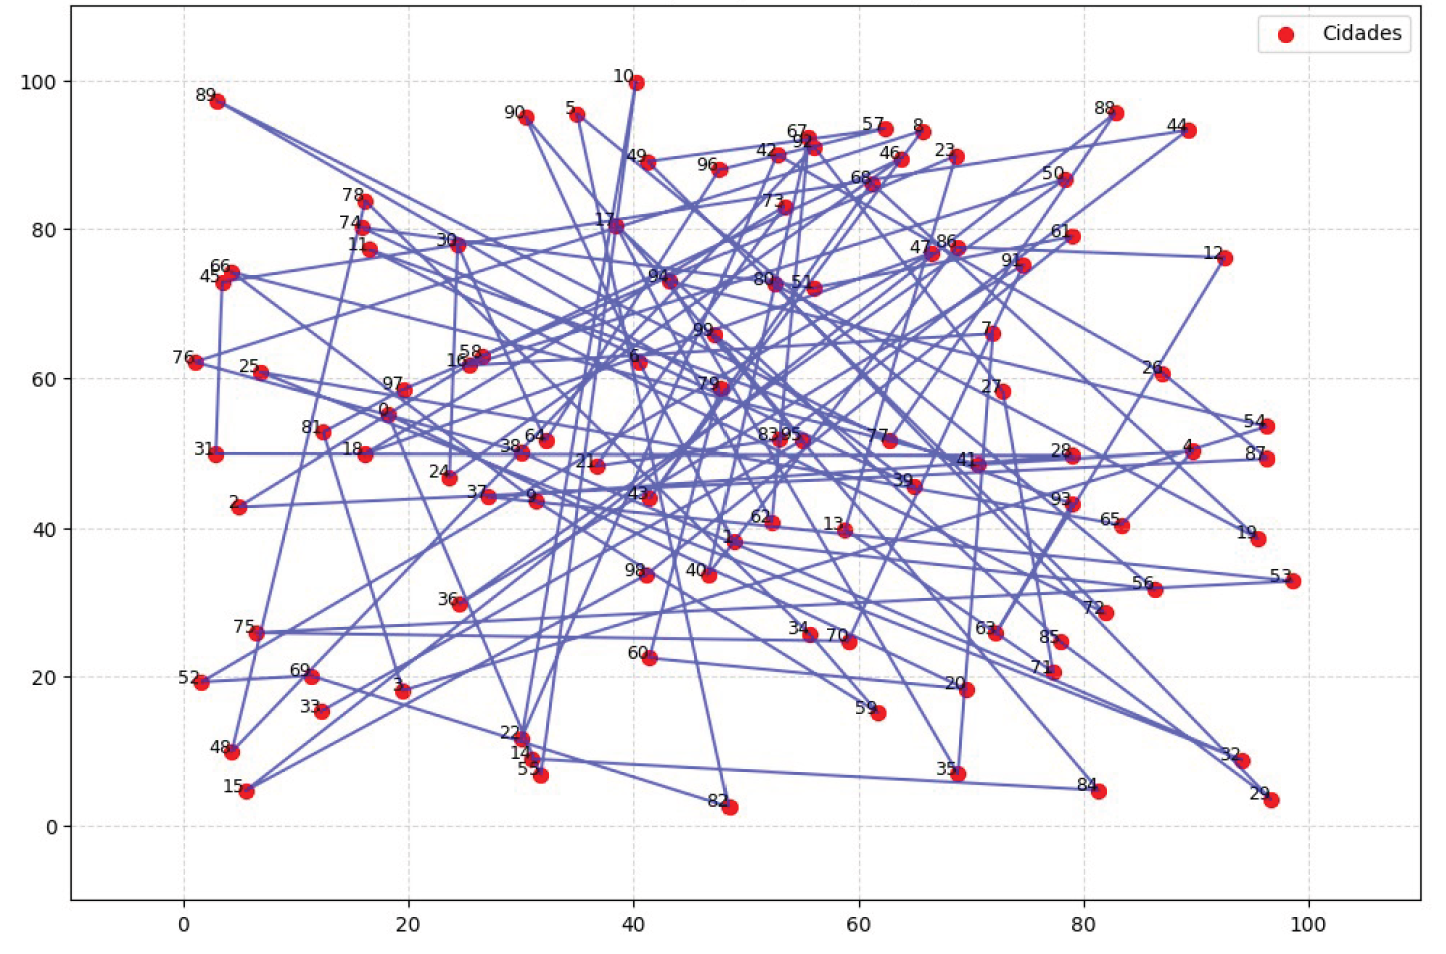
\includegraphics[width=1\linewidth]{apendices/fig/IAA015_2.png}
\caption*{Fonte: O autor (2025).}
\end{figure}

\subsection*{\textbf{2 Compare a representação de dois modelos vetoriais}}

Importações

\begin{lstlisting}[language=Python, style=input]
import numpy as np
import matplotlib.pyplot as plt
from sklearn.feature_extraction.text import TfidfVectorizer
from sklearn.decomposition import PCA
\end{lstlisting}

Trechos de texto
\begin{lstlisting}[language=Python, style=input]
textos = [ 
    "Um mago nunca se atrasa, nem se adianta. Ele chega exatamente quando pretende chegar, pois o tempo dos magos não é o mesmo dos homens. Quando ele chega, é o momento certo.", 
    "Mesmo a menor das pessoas pode mudar o curso do futuro. O que importa não é o tamanho ou a força, mas a coragem que se tem de seguir um caminho que poucos ousariam.", 
    "Tudo o que temos de decidir é o que fazer com o tempo que nos é dado. O que está em nossas mãos, ao fim das contas, é como escolhemos usar os momentos que temos para afetar o que está à nossa volta.", 
    "A jornada não termina aqui. A morte é apenas outro caminho, que todos temos que trilhar. Cada um de nós, por mais que deseje evitar, um dia terá que enfrentar o fim, mas o que fazemos enquanto vivemos é o que realmente importa.", 
    "O mundo não está em seus livros e mapas. Ele está lá fora, nas montanhas, nas florestas e nas planícies. Não se limita ao que você pode ver com os olhos, mas ao que você está disposto a explorar e descobrir.", 
    "Os dias passam como folhas ao vento, mas nossas escolhas permanecem. O que fizemos e as decisões que tomamos, seja na alegria ou na dor, ecoam por todo o nosso caminho e deixam uma marca no que está por vir."
]
\end{lstlisting}

Vetorização TF-IDF

\begin{lstlisting}[language=Python, style=input]
vetorizador = TfidfVectorizer()
X = vetorizador.fit_transform(textos).toarray()
\end{lstlisting}

Redução de dimensionalidade para visualização

\begin{lstlisting}[language=Python, style=input]
pca = PCA(n_components=2)
X_pca = pca.fit_transform(X)
\end{lstlisting}

Plotagem dos vetores

\begin{lstlisting}[language=Python, style=input]
plt.figure(figsize=(8, 6))
plt.scatter(X_pca[:, 0], X_pca[:, 1], color='blue')
for i, txt in enumerate(textos):
    plt.annotate(f"Trecho {i+1}", (X_pca[i, 0], X_pca[i, 1]))
plt.xlabel("Componente Principal 1")
plt.ylabel("Componente Principal 2")
plt.title("PCA dos Textos")
plt.show()
\end{lstlisting}

\begin{figure}[H]
\centering
\caption{PCA dos Textos}
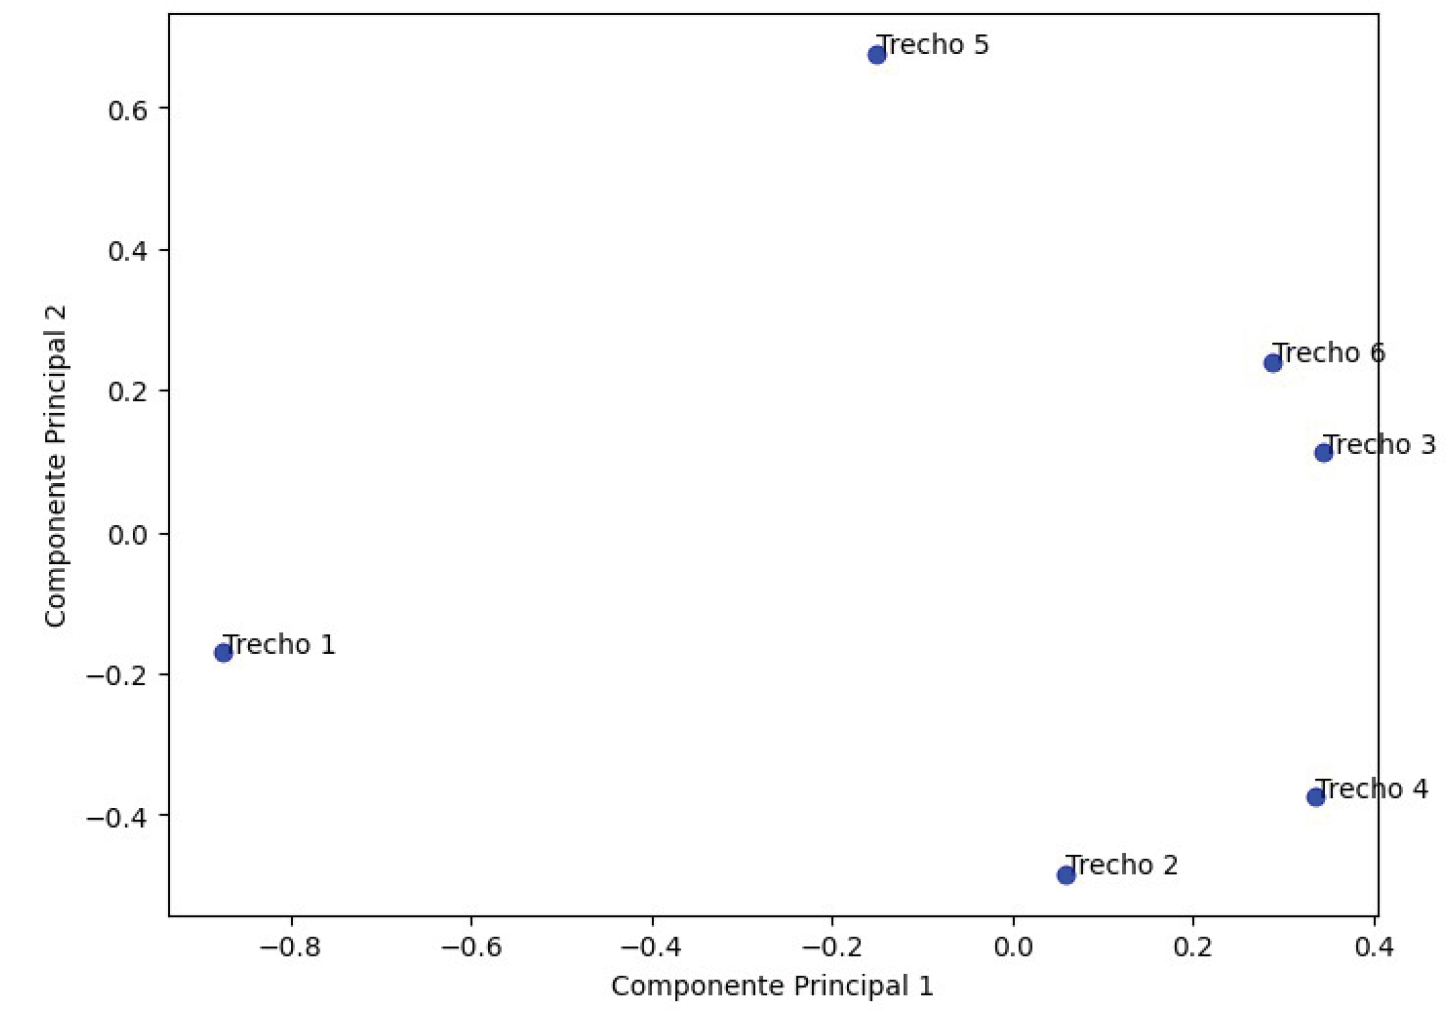
\includegraphics[width=1\linewidth]{apendices/fig/IAA015_3.png}
\caption*{Fonte: O autor (2025).}
\end{figure}

No gráfico, os trechos 3 ("Tudo o que temos de decidir é o que fazer com o tempo que nos é dado...") e 6 ("Os dias passam como folhas ao vento, mas nossas escolhas permanecem...") ficaram bem próximos, o que faz sentido visto que tratam da mesma ideia sobre a importância das escolhas.

Já os trechos 2 ("Mesmo a menor das pessoas pode mudar o curso do futuro...") e 4 ("A jornada não termina aqui. A morte é apenas outro caminho, que todos temos que trilhar...") estão ligeiramente próximos, e isso também faz sentido. Da para entender que ambos os trechos tem um toque de esperança.

Essas similaridades revelam como a representação vetorial consegue captar certos significados em trechos de textos.